%%% AG-BV Template f�r Studien- und Diplomarbeiten %%%

% Doppelseitig: Double sided
%\documentclass[12pt,a4paper,german,twoside,openright]{report}
\documentclass[12pt,a4paper,german,twoside,openright]{report}

% Einseitig: One Sided
%\documentclass[12pt,a4paper,english]{report}

%\usepackage{xr}
%\externaldocument{Fundamental}

\usepackage{jhu_a4}
\usepackage{float}
\usepackage{morefloats}
% SIV-/KT-Symbole -- SIV-/KT-Symbol
\usepackage{ntinclude}

% Sprachunterst�tzung -- Language Imports
\usepackage[english]{babel}

% Bedingungen -- Extra Parameter Conditions
\usepackage{ifthen}

% Allow inserting pdf pages
\usepackage{pdfpages}

\usepackage{makecell}

% Appendencies
\usepackage[titletoc]{appendix}

% TIKZ
\usepackage{tikz}
\usepackage{tikz,amsmath}
\usepackage{tikz-3dplot}
\usetikzlibrary{shapes,calc,positioning}
\usetikzlibrary{calc,intersections}


% Nice citations
\usepackage[square]{natbib}

% Umlaute
\usepackage[latin1]{inputenc}

% Figures k�nnen in Subfigures unterteilt werden
% Figures Can be subdivide into subfigures here:

%\usepackage{subfigure}   
\usepackage{subcaption} 

% Unterst�tzung f�r mehrseitige Tabellen
% Support for multipage tables:
\usepackage{supertabular}

% Zugriff zu Kopf- und Fu�zeilen
% Header and Footers Goes here:
\usepackage{fancyhdr}

% Setzen des Zeilenabstandes
% Settings for line spacing
\usepackage{setspace}
\setstretch{1.2}

% Grafik-Paket -- Graphics Package
%\usepackage[dvips]{graphicx}
%\DeclareGraphicsExtensions{.eps}
\usepackage{graphics}
\usepackage{graphicx}
\usepackage{longtable}
\usepackage{epstopdf}


% Formeln -- Methods(Formulas)
\usepackage{amsmath}
\usepackage{amssymb}


% Sonderzeichen -- Special Characters
\usepackage{marvosym}
\usepackage{wasysym}
\usepackage{textcomp} % for �

\usepackage[calc]{picture}

\let\Setlength\setlength % <--- Important: place this line before loading calc
\usepackage{calc}
\newlength{\arrayrulewidthOriginal}
\newcommand{\Cline}[2]{%
  \noalign{\global\Setlength{\arrayrulewidthOriginal}{\arrayrulewidth}}%
  \noalign{\global\Setlength{\arrayrulewidth}{#1}}\cline{#2}%
  \noalign{\global\Setlength{\arrayrulewidth}{\arrayrulewidthOriginal}}}
 

\setlength{\parindent}{0em}
\setlength{\parskip}{1ex}

\usepackage[linkcolor=black,urlcolor=black]{hyperref}
\usepackage{wrapfig}
%\usepackage{pdfmarginpar} % allows comments
% Key Annotation								\pdfmarginpar[Key]{Key}
% Note Annotation								\pdfmarginpar[Note]{Note}
% Help Annotation								\pdfmarginpar[Help]{Help}
% NewParagraph Annotation				\pdfmarginpar[NewParagraph]{NewParagraph}
% Paragraph Annotation					\pdfmarginpar[Paragraph]{Paragraph}
% Insert Annotation							\pdfmarginpar[Insert]{Insert}

\usepackage{listings} 
\usepackage{color}

\definecolor{lightgray}{gray}{.95}

\lstset{language=C++, showspaces=false, backgroundcolor=\color{lightgray}, tabsize=2, basicstyle=\footnotesize\sffamily, showstringspaces=false, numbers=left, captionpos=b} 


\usepackage[T1]{fontenc}
\usepackage{lmodern}

%% SI unit symbols like degree
%\usepackage{siunitx}
\usepackage{gensymb}

%%%%%%%%%%%%%%%%%%%%%%%%%%%%%%%%%%%%%%%%%%%%%%%%%%%%%%%%%%%%%%%%%%%%%%%%%%%%%%%%%%%%%%%%%%%%%%%%%%%%%%%
% set these to 'black' before printing.
\hypersetup{colorlinks=true,citecolor=black,linkcolor=black}

%%%%%%%%%%%%%%%%%%%%%%%%%%%%%%%%%%%%%%%%%%%%%%%%%%%%%%%%%%%%%%%%%%%%%%%%%%%%%%%%%%%%%%%%%%%%%%%%%%%%%%%
\setcounter{tocdepth}{2} 
\setcounter{secnumdepth}{4} 


%% GENERAL VARIABLES FOR TITLEPAGE ETC. %%%%%%%%%%%%%%%%%%%%%%%%%%%

% Titel der Diplomarbeit oder Studienarbeit
% title goes here:
\newcommand{\SADATitel}{Title}
% Vor- und Nachname -- Names 
\newcommand{\SADAStudent}{Name}
% Diplom- bzw Studienarbeitsnummer
\newcommand{\SADANummer}{Project Group}


% Dokumentanfang
\begin{document}

\tdplotsetmaincoords{90}{90}
% Titelseite
\renewcommand{\textfraction}{0.0001}
\renewcommand{\topfraction}{0.9999}
\renewcommand{\bottomfraction}{0.9999}
%\setcounter{totalnumber}{10}
\setcounter{topnumber}{10}
%\setcounter{bottomnumber}{10}
\setcounter{page}{0}
\pagenumbering{Roman}
\thispagestyle{empty}


\begin{titlepage}

\begin{center}

\textsc{ \Large TECHNICAL UNIVERSITY DORTMUND}\\
\rule[0cm]{0cm}{0.8cm}
{\large Faculty of Electrical Engineering and Information Technology}\\

\rule[0cm]{0cm}{4.75cm}
\SADANummer\\ 

\vspace{1em}


\hspace{-0.0cm}\textbf{\large\SADATitel}\\
\rm
\normalsize

\vspace{1em}

\SADAStudent\\

\rule[0cm]{0cm}{4.75cm}

\textsf{Image Analysis Group\\ Prof. Dr. rer. nat. Christian W{\"o}hler}

\end{center}
\end{titlepage}

\pagestyle{empty}



\section*{Abstract} 



% Seitenstil anpassen
\fancypagestyle{plain}{
% Alte Werte l�schen
\fancyhead{}
\fancyfoot{}

% Seitennummer oben rechts (ungerade Seite) bzw. oben links (gerade Seite)
% Page number top right (odd side) or top left (straight side)
\fancyhead[RO,LE]{\thepage}

% Abschnittsnummer auf ungerader Seite oben links
% Section number on the odd-numbered page in the upper left corner
\fancyhead[LO]{\rightmark}

% Kapitelnummer auf gerader Seite oben rechts
% Chapter number on straight side in the upper right
\fancyhead[RE]{\leftmark}

% Kopfzeile unterstreichen
% Headline underline
\renewcommand{\headrulewidth}{\iffloatpage{0pt}{0.4pt}}
\headheight 15pt}
\pagestyle{plain}
\renewcommand{\chaptermark}[1]{\markboth{\textsc{\thechapter}.\ \textsc{#1}}{}}
\renewcommand{\sectionmark}[1]{\markright{\thesection\ #1}}

% Inhalts- und Abbildungsverzeichnis
\setcounter{page}{1}
\pagenumbering{Roman}
\tableofcontents
\clearpage{\pagestyle{empty}\cleardoublepage}

\setcounter{page}{1}
\pagenumbering{arabic}

%%%%%%%%%%%%%%%%%%%%%%%%%%%%%%%%%%%%%%%%%%%%%%%%%%%%%%%%%%%%%%%%%%%%%%%%%%%%%%%%%%%%%%%%%%%%%%%%%%%%%%%
%%%%%%%%%%%%%%%%%%%%%%%% Inhalt erg�nzen %%%%%%%%%%%%%%%%%%%%%%%%%%%%%%%%%%%%%%%%%%%%%%%%%%%%%%%%%%%%%%



\chapter{Motivation}

\chapter{Fundamentals}
\section{Datasets}
\subsection{Mars2020 Mission Information}
\subsubsection{Cameras}
\paragraph{Navigation Camera}
\label{navigationCamera}

The Navigation camera(Navcam) is a mast-mounted stereo pair of engineering cameras which are seperated by a baseline lenght of 42.4cm. They are designed to survey the terrain around the rover by acquiring images from atop a pan/tilt mast mounted on the top deck of the rover with a $360\degree$ field of the terrain. It is located at the RSM head, co-boresighted with the Mast Camera.
\begin{figure}[H]
	\centering
	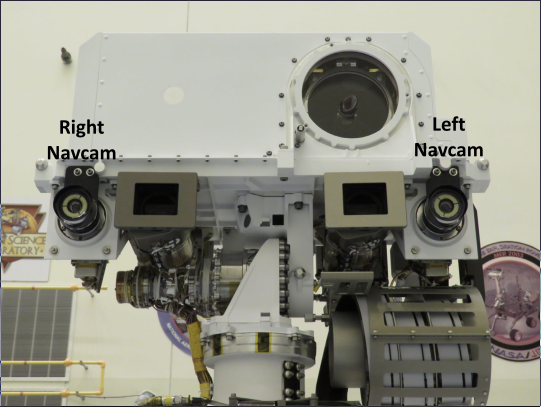
\includegraphics[scale=0.5]{img/locationNavcams.png}
	\caption{Navcam Location}
	\label{fig:navcamLocation}
\end{figure}
The Navcam images are used for traverse planning, general site characterization(panoramic images and targeted images of interest, including terrains that are not viewable by the Hazard Avoidance Camera), target identification and selection, robotic arm operation and rover auto-navigation. The Navcams are also used to monitor and document the state of the vehicle by acquiring images of the rover harware and determine the rover attitude in the local Mars frame by acquiring images of the sun. The label of the images taken by Navcam starts with 'NL' and 'NR' identifiying the left and the right Navcam images. 

\begin{table}[H]
	\centering
	\caption{Navcam Characteristics}
	\label{tab:navcamChar}
	\begin{tabular}{ | p{5cm} | p{5cm} | } 
  \hline
  Optics                             & Description\\
  \hline
  Horizontal FOV                     & 96\degree\\
  Vertical FOV                       & 73\degree \\
  Diagonal FOV                       & 120\degree \\
  Focal Ratio                        & $f/12$\\
  Best Focus                         & 3.5 meters\\
  Stereo Baseline                    & 42.4$m$\\
  Angle between left/right boresight & $<0.4\degree$(parallel)\\
  Boresight mounting orientation     & Mounted to pan/tilt RSM, left/right camera boresights are parallel.\\
  Height above nominal surface       & approx. 1.98 meters viewing the horizon.\\
  Pixel Format                       & 5120 x 3840\\
  Pixel pitch                        & 6.4 \textmu m x 6.4 \textmu m\\
  Optical format                     & Full frame(32.77 mm x 24.58mm)\\
  \hline
	\end{tabular}
\end{table}

\paragraph{Mast Camera Zoom}
\label{mastCameraZoom}

The Mastcam-Z is a multispectral, stereoscopic imaging investigation device on the Mars 2020 mission's Perseverance rover. Each Mastcam-Z camera consists of a 1648 x 1214 pixel charge-shift detector and electronics, in addition to zoom, focus and filter wheel mechanisms. The two Mastcam-Z cameras are mounted on a rover reconnaissance mast with a 24.4 cm stereo baseline and have a total 2.3\degree toe-in on the camera plate approximately 2m from the surface that provides azimuth and elevation triggers. 
\begin{figure}[H]
	\centering
	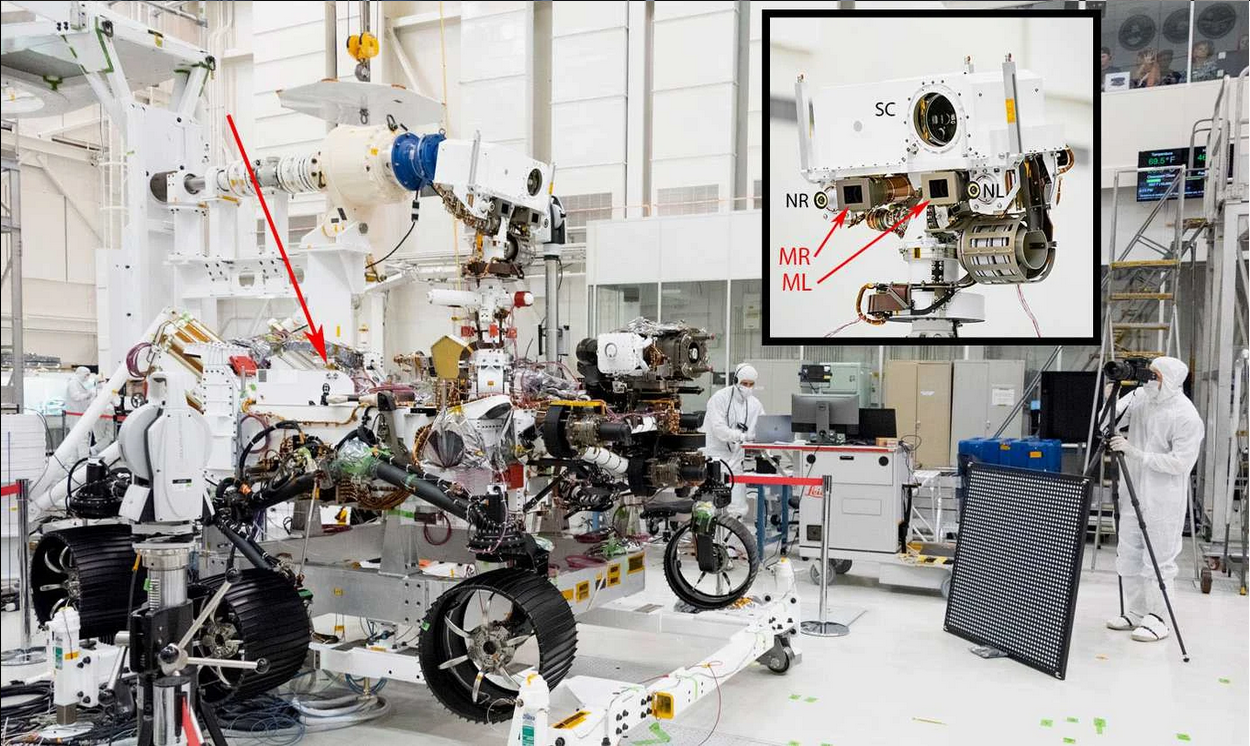
\includegraphics[scale=0.3]{img/mastcamlocation.png}
	\label{fig:mastcamLocation}
	\caption{Location of MastcamZ}
\end{figure}
Primary and secondary MastcamZ calibration targets mounted on the rover's upper deck allow for tactical reflectance calibration. It uses Mastcam-Z's multispectral, stereo and panoramic imagery to provide detailed morphological, topographical and geological context along the rover's traverse. Limit the mineralogical, photometric and physical properties of surface materials. Monitoring and characterization of atmospheric and astronomical phenomena. Document rover sample extraction and cache locations. Mastcam Z images  also provide important technical information to support sample selection and other rover drive and tool equipment operation decisions.

\begin{table}[H]
	\centering
	\caption{Mastcam Characteristics}
	\label{tab:mastcamChar}
	\begin{tabular}{ | p{5cm} | p{5cm} | } 
  \hline
  Optics                 & Description\\
  \hline
  Focus                  & Adjustable, Working distance $0.5-1.0 m to \infty$ \\
  FOV(1600 x 1200 pix)   & 25.6\degree x 19.2\degree Widest and 6.2\degree x 4.6\degree Narrowest\\
  Focal ratio            & f/6.7 and f/9.5\\
  Effective focal length & 26 mm and 110 mm\\
  Array size             & 1600 x 1200 photoactive pixels ( 1648 x 1214 total)\\
  Pixel size             & 7.4\textmu (square pixels)\\
  Stereo baseline        & 24.4 cm; toe-in angle between cameras; 2.3\degree\\
  \hline
	\end{tabular}
\end{table}




%Refernce
%
%[1]https://pds-geosciences.wustl.edu/m2020/urn-nasa-pds-mars2020_mission/document_camera/Mars2020_Camera_SIS.pdf
%
%[2]https://www.vrvis.at/publications/pdfs/PB-VRVis-2021-025.pdf)
%
%[3][mastcam](https://link.springer.com/article/10.1007/s11214-020-00755-x)


%[2]improvment of the cameras from the MSL in the perseverance rover.
%Navcam FOV was too narrow, limited assement of the vehicle state due to the lack of color information
%lower angular pixel scale

\subsubsection{Stereo Vision}
\paragraph{Homogeneous Coordinates}
Homogeneous coordinates is a coordinates system used in projective geometry which serve as an alternate for Eculidian expression for geometric objects and transofrmations. Incase of Euclidian system it becomes suboptimal when we describe central projections and makes the caluculation of transofrmations complex. In a pinhole camera model a object is mapped from 3D to a 2D image. There are different types of mappings done to preserve specific geometric aspect(straight lines, angles and size). To map the 2D coordinates to 3D coordinates we need to perform transofrmations with the 2D coordinates. This becomes difficult to describe the translation with a matrix in Euclidian space ae it describe linear transofrmations. Hence we use homogeneous coordinates where we can express a varaiety of transofrmations. If homogeneous coordinates of a geometric object x is multiplied by a non-zero scalar then the resulting coordinates represent the same point.
\begin{equation}
	x = \lambda x
\end{equation}
Homogeneous coordinates uses a $n +1$ dimesion vector to represent a $n$ dimesion eculidian vector. 
\begin{equation}
x = 
	\begin{bmatrix}
		x \\
		y 
	\end{bmatrix}
x = 
	\begin{bmatrix}
		x \\
		y \\
		1
	\end{bmatrix}
	= 
	\begin{bmatrix}
		wx \\
		wy \\
		w
	\end{bmatrix}
	= 
	\begin{bmatrix}
		u \\
		v \\
		w
	\end{bmatrix}
\end{equation}

Homogeneous coordinates allows the possibility of matrix operations, such that all chain transofrmations can be represent by matrix multiplication. The points that are located at infinity can be expressed with finite coordinates. This allows us to represent affine and projective transofrmations with a single matrix.

%[1](https://en.wikipedia.org/wiki/Homogeneous_coordinates)


\paragraph{Calibrated vs Uncalibrated Reconstruction}
In claibrated reconstruction we use the image plane coordinates, here the intrinsic and the extrinsic parameters are known. These parameters are used to rectify the images The epipolar geometry reduces the correspondance problem to a line search problem. We implement a template matching method to find the stereo correspondance, from which we can obtain the disparity calcualtion. The disparity map is used to obtain the points in the 3D space, which allows us to recreate the object. 

Uncalibrated Reconstruction does not have the knowladge of the camera parameters, they are estimated. We use feature matching methods to find unique image points for both the stereo images and find the fundamental matrix F using the least square method. The essential matrix is calculated from the fundamental matrix, in which we use SVD to get the rotation matrix and the translation matrix. After estimating the parameters the uncalibrated reconstruction follows the calibrated method. Where we find the correspondance using template matching to obtain the disparity map, which is used to calculated the 3D coordinates for the reconstructed object. The pipeline of calibrated and the uncalibrated method is explained in detail in the implementation section.


\section{Methods}

\newpage
\chapter{Implementation}
\section{Reconstruction from Rover Images}
%tikzstyle
\tikzstyle{decision} = [diamond, draw, fill=blue!20, 
text width=6em, text badly centered, node distance=3cm, inner sep=0pt]
\tikzstyle{block} = [rectangle, draw, fill=blue!20, 
text width=6em, text centered, rounded corners, minimum height=2em]
\tikzstyle{block2} = [rectangle, draw, fill=yellow!20, 
text width=9em, text centered, rounded corners, minimum height=4em]
\tikzstyle{line} = [draw, -latex']
\tikzstyle{cloud} = [draw, ellipse,fill=red!20, node distance=3cm,
minimum height=4em]

In our project we used the open source computer vision library(Opencv) to perform 3D Reconstruction. We implemented both calibrated and Uncalibrated stereo reconstruction techniques using opencv. Opencv uses a pinhole camera model[ref] which works by projecting 3D points onto the image plane using a perspective transformation.

\paragraph{Callibrated}

In calibrated reconstruction the parameters were calculated form the .xml files provided with the images. We used the calculation method followed by \cite{CHAVOREcalculation}, which was implemented as a pyhton script by \cite{CHAVOREcalculation}. For the Callibrated reconstruction we followed the \ref{pipe:calibratedOpencv} pipeline in opencv.


\begin{figure}[H]
	\centering
	\begin{tikzpicture}[node distance = 2cm, auto]
		\node [block] (init) {Input stereo Images};
		\node [block, right of = init, node distance = 3.5cm] (rectify) {Stereo Rectification};
		\node [block, right of = rectify, node distance = 3.5cm] (undistort) {Undistortion Map};
		\node [block, right of = undistort, node distance = 3.5cm] (matching) {Stereo Matching};
		\node [block, right of = matching, node distance =3.5cm] (disp) {Disparity calculation};
		\node [block, above of = disp, node distance = 2cm] (cloud) {Poin Cloud};
		\node [block, below of = disp, node distance = 2cm] (depth) {Depth Map};
		\path [line] (init) -- (rectify);
		\path [line] (rectify) -- (undistort);
		\path [line] (undistort) -- (matching);
		\path [line] (matching) -- (disp);
		\path [line] (disp) -- (cloud);
		\path [line] (disp) -- (depth);
	\end{tikzpicture}
	\label{pipe:calibratedOpencv}
	\caption{Opencv Callibrated pipeline}
\end{figure}

The camera parameters are then used to form the camera matrix, the distortion coefficients and extrinsic matrices. To perform rectification we use \emph{cv2.stereoRectify} function in Opencv which takes thes matrices as inputs and gives the rectified rotation for the left and the right image planes, the left and the right projection equation and the reprojection matrix $Q$. The rectified parameters are then used to create a stereo map for both the images with \emph{cv2.initUndistortRectifyMap} function where we get a Undistortion map for the images. These maps are then given as inputs to \emph{cv2.remap} function where we get the undistorted images as the output.

\begin{lstlisting}[language=python, caption=Rectification and Undistortion]

#Rectification
rectL, rectR, projMatrixL, projMatrixR, QR= cv.stereoRectify(
params.cameraMatrixL, params.distL,params.cameraMatrixR,
params.distR, shapeR, params.extrinscis['R'], params.extrinscis['T'])
	
#Undistortion
stereoMapL = cv.initUndistortRectifyMap(params.cameraMatrixL,
params.distL, rectL, projMatrixL, shapeL, cv.CV_16SC2)
stereoMapR = cv.initUndistortRectifyMap(params.cameraMatrixR,
params.distR, rectR, projMatrixR, shapeR, cv.CV_16SC2)

imgL = cv.remap(self.imageL, stereoMapL[0], stereoMapL[1],
cv.INTER_LANCZOS4, cv.BORDER_CONSTANT, 0)
imgR = cv.remap(self.imageR, stereoMapR[0], stereoMapR[1],
cv.INTER_LANCZOS4, cv.BORDER_CONSTANT, 0)

\end{lstlisting}

The next step involves stereo matching where we implement block matching between the stereo pairs. We first create a block matching object with specific parameters form trail and error. The object is then used to cmpute the disparity map using the \emph{compute} function with the object. To get the 3D points form the disparity map we use the \emph{cv.reprojectImageTo3D} function which takes the disparity map and the reprojection matrix as input to give the 3D points. These points then can be saved as .ply file for viewing.

\begin{lstlisting}[language=python, caption=Disparity Map and Reprojection]
# Create Block matching object. 
stereo = cv.StereoSGBM_create(minDisparity= min_disp,
	numDisparities = num_disp,
	blockSize = block_size,
	uniquenessRatio = 5,
	speckleWindowSize = 5,
	speckleRange = 2,
	disp12MaxDiff = 2,
	P1 = 8 * 3 * block_size**2,
	P2 = 32 * 3 * block_size**2)

#Create Disparity Map
disparity_map = stereo.compute(grayL, grayR)

#Get 3D points
points_3D = cv.reprojectImageTo3D(disparity_map, Q, handleMissingValues=False)

\end{lstlisting}

\paragraph{Uncalibrated}

Uncalibrated reconstruction in Opencv tries to estimate the parameters by using feature matching techniques. It follows the \ref{pipe:uncalibratedOpencv} pipeline where we first use SIFT to detect the keypoints from the stereo images and extract the matching descriptiors using enchanced nearest neighbour method. We then used the lowes test to filter the match with a specific threshold.

\begin{figure}[H]
	\centering
	\begin{tikzpicture}[node distance = 2cm, auto]
		\node [block] (init) {Input stereo Images};
		\node [block, right of = init, node distance = 3.5cm] (keypoints) {Detect Kepoints};
		\node [block, right of = keypoints, node distance = 3.5cm] (match) {Match Descriptors};
		\node [block, right of = match, node distance =3.5cm] (rect) {Rectification};
		\node [block, below of = rect, node distance = 2cm] (disparity) {Disparity};
		\node [block, left of = disparity, node distance = 3.5cm] (3dpoints) {Point Cloud};
		\path [line] (init) -- (keypoints);
		\path [line] (keypoints) -- (match);
		\path [line] (match) -- (rect);
		\path [line] (rect) -- (disparity);
		\path [line] (disparity) -- (3dpoints);
	\end{tikzpicture}
	\label{pipe:uncalibratedOpencv}
	\caption{Opencv UnCallibrated pipeline}
\end{figure}

\begin{lstlisting}[language=python, caption=Feature matching]
sift = cv.SIFT_create()
key1, desc1 = sift.detectAndCompute(image_left, None)
key2, desc2 = sift.detectAndCompute(image_right, None)

#FLANN Enhanced Nearest Neighbour Method
FLANN_INDEX_KDTREE = 1
index_params = dict(algorithm = FLANN_INDEX_KDTREE, trees = 5)
search_params = dict(checks=50)
flann = cv.FlannBasedMatcher(index_params,search_params)
Flann_matches = flann.knnMatch(desc1,desc2,k=2)

\end{lstlisting}

The \emph{cv2.stereoRectifyUncalibrated} function is used to get the homography matrices for the images, which is used with \emph{cv2.warpPerspective} to get a rectified image. The disparity for the rectified image is calculated with block matching. We create a reprojection matrix form the camera parameters(cx, cy, focal length and base line). The \emph{cv2.reprojectImageTo3D} function gives the 3D points from the disparity map and the projection matrix.

\begin{lstlisting}[language=python, caption=Uncalibrated Rectification]
#rectification
_, H1, H2 = cv.stereoRectifyUncalibrated(
    np.float32(pts1), np.float32(pts2), f, imgSize=(w1, h1)
)

imgl_rectified = cv.warpPerspective(image_left, H1, (w1, h1))
imgr_rectified = cv.warpPerspective(image_right, H2, (w2, h2))

#Disparity Calculation
stereo = cv.StereoBM_create(numDisparities=16, blockSize=15)
disparity_BM = stereo.compute(imgl_rectified, imgr_rectified)

#Reprojection
image3d = cv.reprojectImageTo3D(disparity_map, Q, handleMissingValues=False)

\end{lstlisting}

%[opencv](https://docs.opencv.org/4.x/d6/d00/tutorial_py_root.html)
%[chavore]( https://github.com/bvnayak/CAHVOR_camera_model)



\subsection{Metashape}
\subsubsection{Uncalibrated}
%Alignment Process in Metashape
%tikzstyle
\tikzstyle{decision} = [diamond, draw, fill=blue!20, 
text width=6em, text badly centered, node distance=3cm, inner sep=0pt]
\tikzstyle{block} = [rectangle, draw, fill=blue!20, 
text width=6em, text centered, rounded corners, minimum height=2em]
\tikzstyle{block2} = [rectangle, draw, fill=yellow!20, 
text width=9em, text centered, rounded corners, minimum height=4em]
\tikzstyle{line} = [draw, -latex']
\tikzstyle{cloud} = [draw, ellipse,fill=red!20, node distance=3cm,
minimum height=4em]


\paragraph{Alignment}
\label{alignment}

The alignment is the first step in the reconstruction process in agisoft metashape. This step can be broken down into different stages when we reconstruct the region of intrest.
\begin{figure}[!ht]
	\centering
	\begin{tikzpicture}[node distance = 2cm, auto]
		\node [block] (init) {selection of images};
		\node [block, right of = init, node distance = 4cm] (mask) {applying masks};
		\node [block, right of = mask, node distance = 4cm] (markers) {placing markers};
		\node [block, right of = markers, node distance = 4cm] (alignment) {alignment of images};
		\path [line] (init) -- (mask);
		\path [line] (mask) -- (markers);
		\path [line] (markers) -- (alignment);
	\end{tikzpicture}
	\label{pipe:alignment}
	\caption{alignment process}
\end{figure}
\subparagraph{selection of images}
\label{selectionofimages}

In our project we selected the images based on the most visited location by the rover and the amount of time that the rover has spent on that particular region. We decided the region based on the information \cite{locationMap} provided by NASA. By calculating the sols we can infer the number of days the rover has spent on a region from which we can choose a particular range of sols to reconstruct. Since the \cite{pdsNode} contains a plethora of images which will include the claibration target, on-board equipments, images of sun, test images, etc. It will become a tedious process to Identity the images from each sol that can provide us with a good model in the final stages since downloading multiple sols consumes lot of time and at some sols not all images will be required for the reconstruction. We used the \cite{stereoImages} to filter the sols that have good images for the reconstruction. From our work with Agisoft metashape we infered that for a good reconstruction we should provide the images from different views for a single object/rock. So we selected locations that had multiple images form different angles.

\subparagraph{Applying Masks}
\label{applyingMasks}

Metashape provides a tool with which we can mask the unwanted noise/background in the images. We used this feature since somes images had a good description of the object to be reconstructed but hindered by other objects, rover equipments, etc. 

\subparagraph{Placing Markers}
\label{placingMarkers}

Markers are used to interlink one point in a image with another image. This speeds up the alignment process and also points agisoft to align the images based on the markers. Thus by connecting multiple images with the markers we will be able ot get a good reconstruction from the selected images.

\begin{figure}[H]
	\centering
	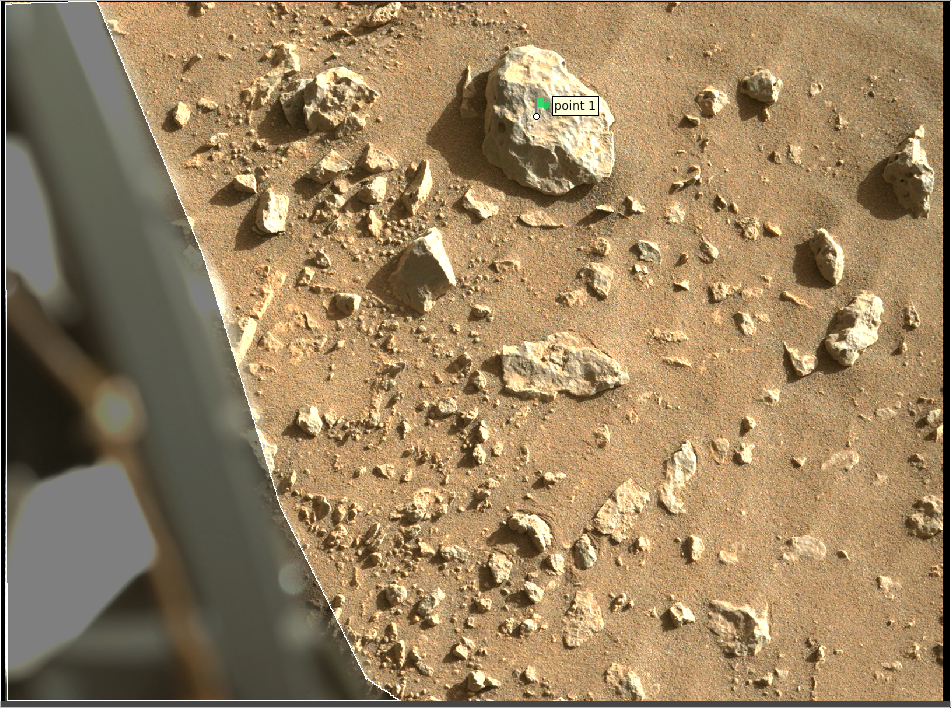
\includegraphics[scale=0.3]{img/masksandMarkers.png}
	\caption{Applying Masks and Markers}
	\label{fig:masksMarkers}
\end{figure}
\subparagraph{Alignment of Images}
\label{alignmentOfImages}
This step performs triangulation and bundle block adjustment. Agisoft searches for feature points across the images and matches them to tie points. It estimates the camera position of each image, also with the intrinsic and the extrinsic camera parameters.\emph{Masks} and \emph{Markers} allows agisoft to searche for feature points in those specific regions. This allows us to ignore the unessential parts for the reconstruction as we work with different cameras with distinct characteristics. While aligning we used the high accurarcy settings and increased the keypoint limit to 40,00. Increasing the accurarcy may provide better results but the time for the alignment will be considerably increased.
\begin{figure}[H]
	\centering
	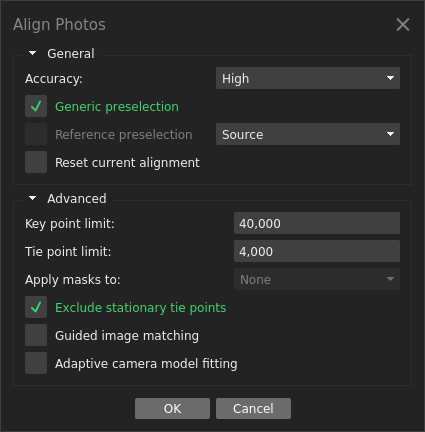
\includegraphics[scale=0.6]{img/alignmet.png}
	\caption{Alignment in Agisoft}
	\label{fig:alignment}
\end{figure}
The output of the alignment process gives the tie points and a set of estimated camera positions. The result of alignment will be determined by the number of images that have been fully aligned as some images tend not to align. The tie points represents the results of the image alignment and also used for the determination of the depth map calculation 


After the creation of the dense point cloud, we can use metashape to create a polygonal mesh model with the point cloud information and the the depth maps data. The \emph{build mesh} command used to create a mesh for the selected point cloud. To get a high quality output we selected the source data to be the dense point cloud, even though it requires a longer processing time. The face count specifies the number of polygonals in the final we used the high settings in our reconstruction to give a quality mesh. The vertex colors are calculated and the depth maps from the alignment process is reused here.\\

\begin{figure}[H]
	\centering
	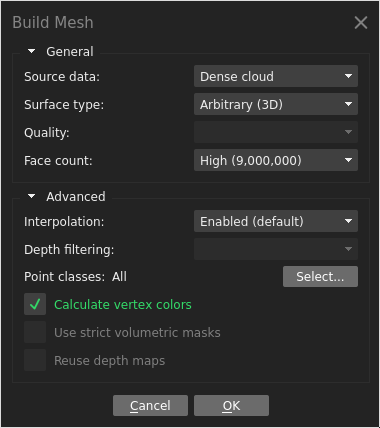
\includegraphics[scale=0.5]{img/mesh.png}
	\caption{Mesh Generation}
\end{figure}
Texture genration in metashape uses the source data from the aligned images which allows it build a color texture map for the model. Metashape also allows to fill holes in the model. We kept the other parameters same as the default standard when building the texture. The texture model that we obtained from metashape had higher quality but they occupied more space with higher the quality.

\begin{figure}[H]
	\centering
	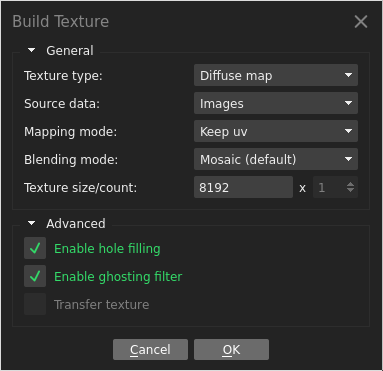
\includegraphics[scale=0.5]{img/texture.png}
	\caption{Texture Generation}
\end{figure}

%[1](https://www.agisoft.com/pdf/metashape-pro_1_8_en.pdf)


\subsubsection{Calibrated}
Agisoft Metashape can approximate the camera parameters automatically, but to get an accurate reconstruction of the object we include the intrinsic camera parameters. The parameters can be given for each image individually or we can create groups of images and impose the same parameters for all the images in the group. The intrinsic parameters are calculated form the CHAVORE[ref] data that is provided for all the images in the $.xml$ files. The parameters are form[ref] which is scripted in python[1]. The input parameters are $f, k1, k2, k3, cx, cy$, as seen in \ref{fig:cameraCalibrationMetashape} which is the focal length, distortion coefficent and the principal point of the images.
\begin{lstlisting}[language=xml, caption=xml file, label=xmlFile]
<?xml version='1.0' encoding='UTF-8'?>
<calibration>
  <projection>frame</projection>
  <width>1648</width>
  <height>1200</height>
  <f>14771.071671547474</f>
  <cx>-0.3312798406959963</cx>
  <cy>1.0928099206940067</cy>
  <k1>0.000193151</k1>
  <k2>1.8354094491035e-09</k2>
  <k3>8.081357601557738e-19</k3>
</calibration>
\end{lstlisting}
\begin{figure}[H]
	\centering
	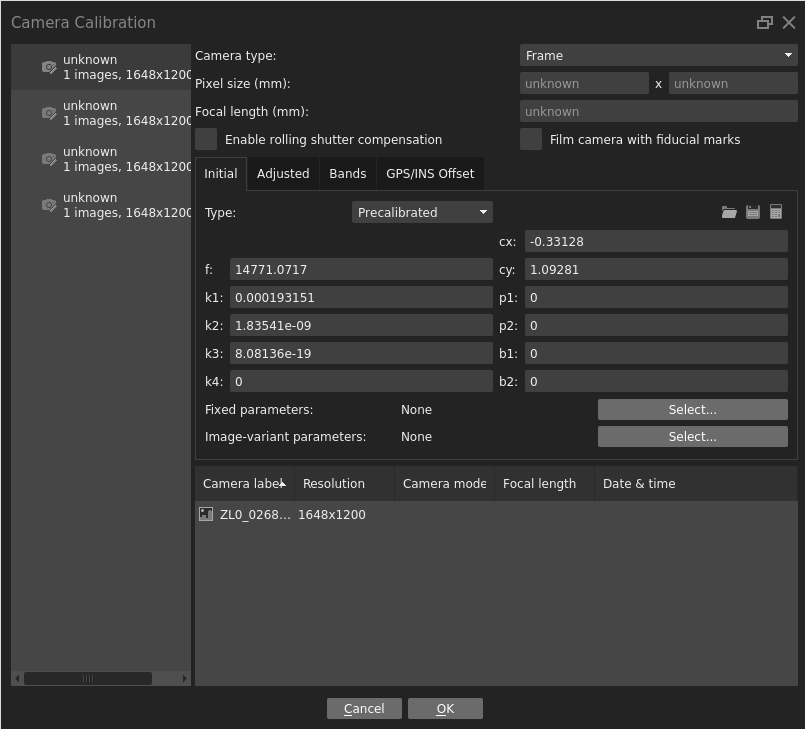
\includegraphics[scale=0.3]{img/cameraCalibration.png}
	\caption{Callibration Parameters}
	\label{fig:cameraCalibrationMetashape}
\end{figure}
These parameters are stored in a $.xml$ file by using a script[ref] that converts the data to xmls, as agisoft allows us to upload the parameters through a file \ref{xmlFile} instead of manually entering all the values. The option to upload the file can be found on \ref{fig:cameraCalibrationMetashape} for each selected image.
\begin{figure}[H]
	\centering
	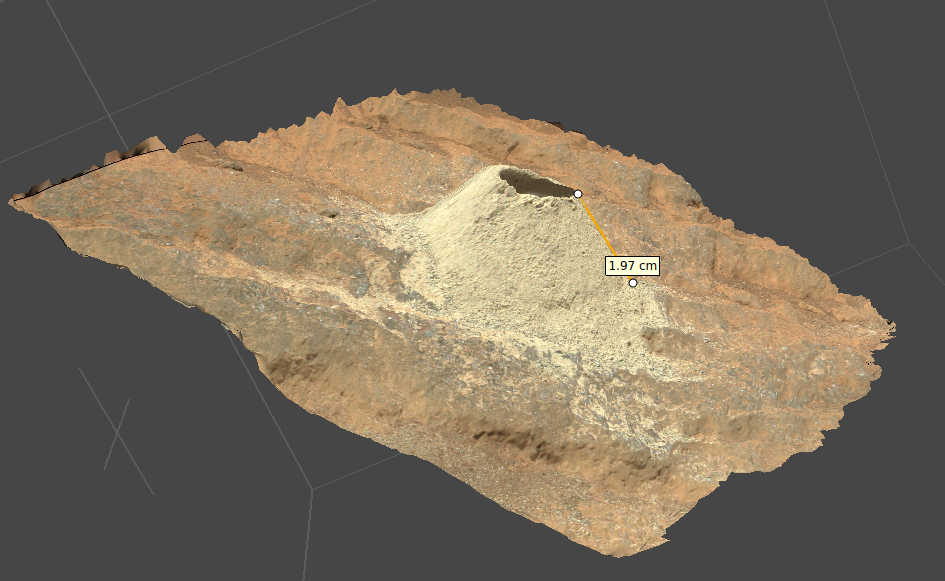
\includegraphics[scale=0.3]{img/drill.png}
	\caption{Sol-268 with Parameters}
	\label{fig:drillHole}
\end{figure}
This makes the alignment process more accurate and the model that we get will be scaled to the actual size of the object as seen in \ref{fig:drillHole}. As in Uncalibrated reconstruction without the parameters we do not get an exact dimesion of the reconstructed object. When dealing with multiple images the process of selecting the xmls for them can be automated with a python script. All processes in agisoft can be maniputed using the python metashape package in a script, this reduces the process of uploading the data for each image when dealing with reconstruction that involves multiple images.



\section{3D Models from Rover Imagery}

\section{Digital Elevation Models from Satellite Imagery}

\section{VR Integration}


\newpage
\chapter{Results}
\section{Rover Group}
\subsection{Metashape}
\subsection{Uncalibrated}

\subsubsection{Sol-185}

This sol was selected by us for reconstruction as it was recogonized as a region of interest with with unique geological makeup. Which led to make the rover spending more time in the area by taking many high quality images using the Mastcam. Arround 108 images were used to reconstruct the scene form sol 180 to sol 188. Thus having multiple view of images provided to be an advantage during reconstruction.

\begin{figure}[H]
	\centering
	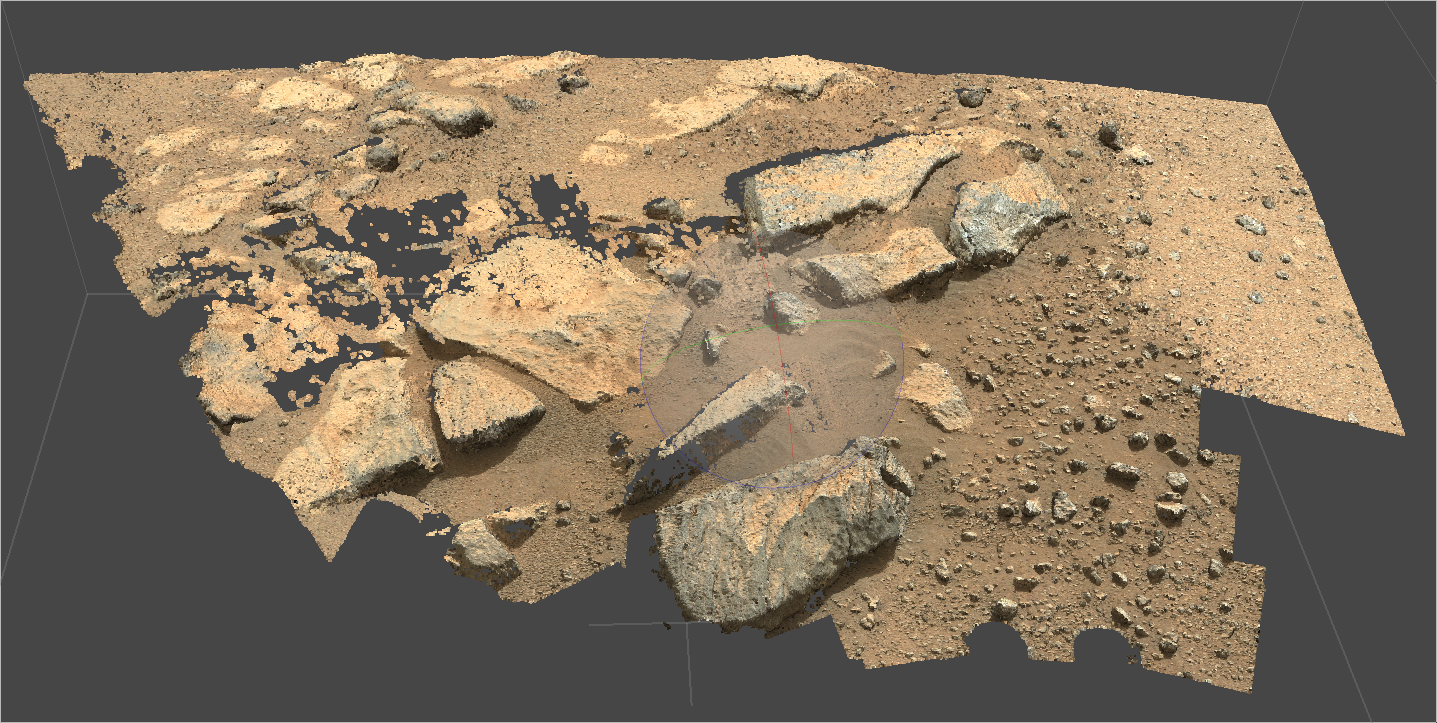
\includegraphics[scale=0.3]{img/sol185.png}
	\label{fig:sol185}
	\caption{}
\end{figure}

\subsubsection{Sol-197}

This rock is named "Rochette" by NASA, as they decided to drill a second time on this rock since it had unique features and geological makeup which was an interest for astrobiology. Thus providing us with 35 Mastcam images of high quality for the reconstruction. The images from sol 197 and sol 198 were used which are the images post boring on the rock. 


\begin{figure}[H]
	\centering
	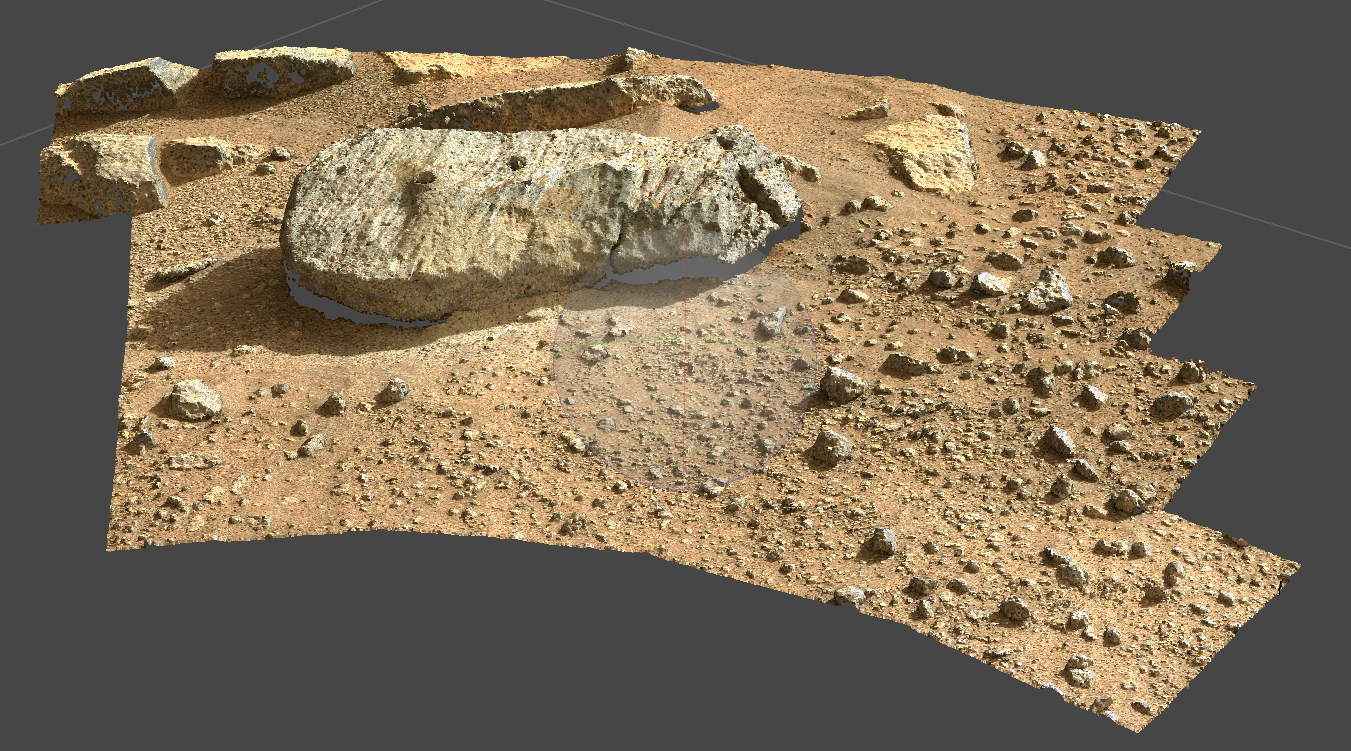
\includegraphics[scale=0.3]{img/sol195.png}
	\label{fig:sol197}
	\caption{}
\end{figure}

\subsubsection{SOl-106}

This location was reconstructed using 118 images. We used the high quality Mastcam images form sol106.

\begin{figure}[H]
	\centering
	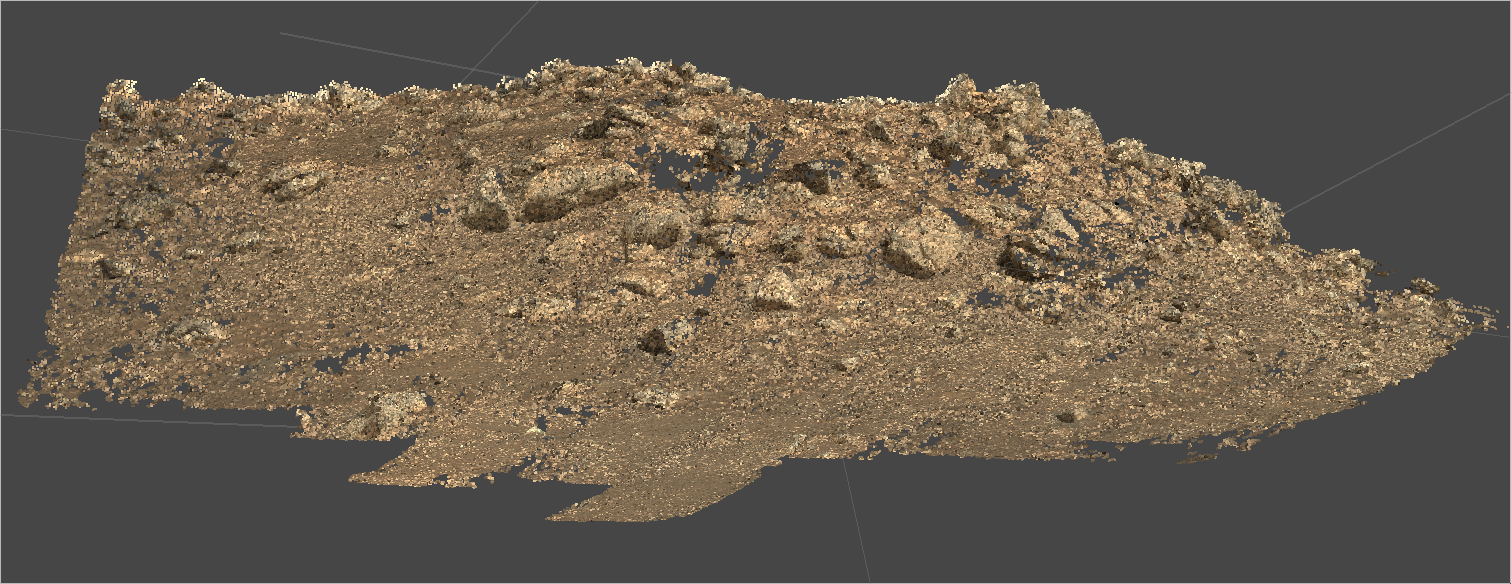
\includegraphics[scale=0.3]{img/sol106pc.png}
	\label{fig:sol103}
	\caption{}
\end{figure}

\subsubsection{Sol-268}
\label{sec:drilluncal}

This location was used to collect a sample for geological purpose. The reconstructed part potrays the drill that was made by the rover. We used 4 images from different angles form Mastcam to give a quality reconstruction.

\begin{figure}[H]
	\centering
	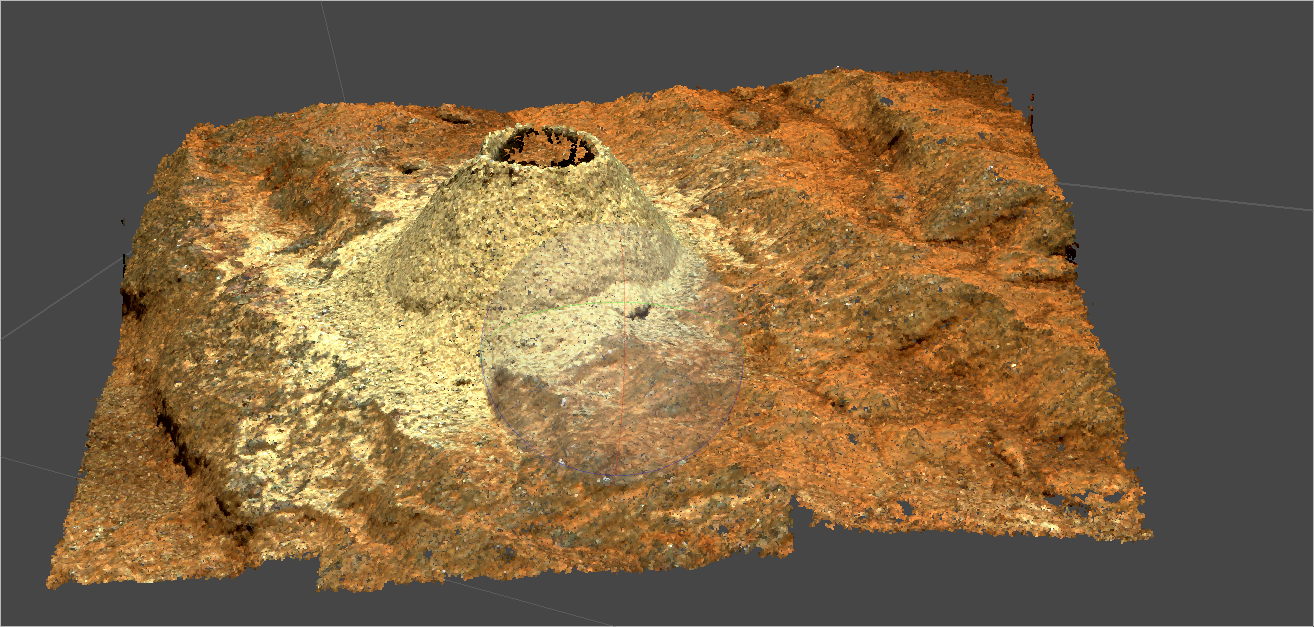
\includegraphics[scale=0.3]{img/sol286.png}
	\label{fig:sol268}
	\caption{}
\end{figure}

\subsubsection{Sol-54}
\label{sec:sol54}

The location had more high quality photos for reconstruction. We used 118 images from the Mastcam to reconstruct the area. 

\begin{figure}[H]

	\centering
	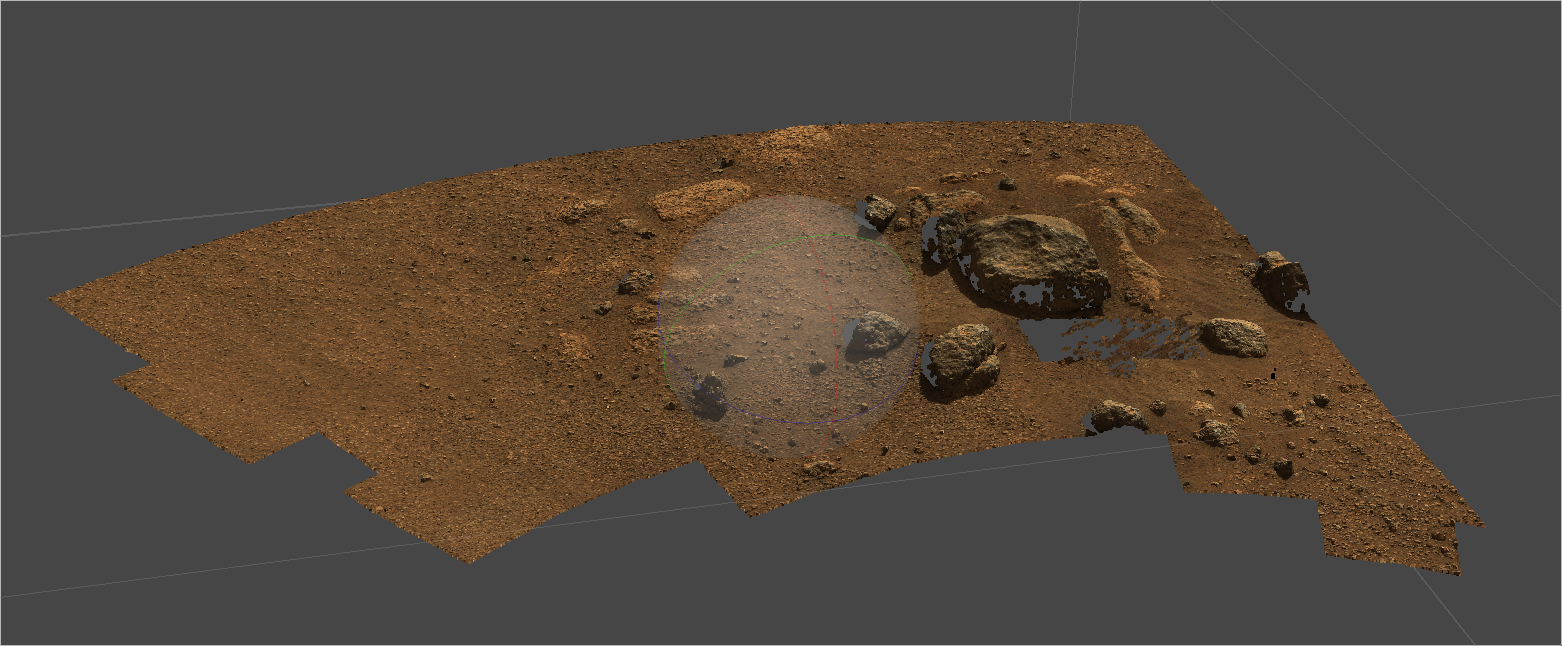
\includegraphics[scale=0.3]{img/sol42.png}
	\label{fig:sol54}
	\caption{}
\end{figure}
\subsubsection{Sol-283}

This location is one of newer area which the rover was exploring at the time, which had many features. This reconstruction was done by us using 8 images from the Mastcam.
\begin{figure}[H]
	\centering
	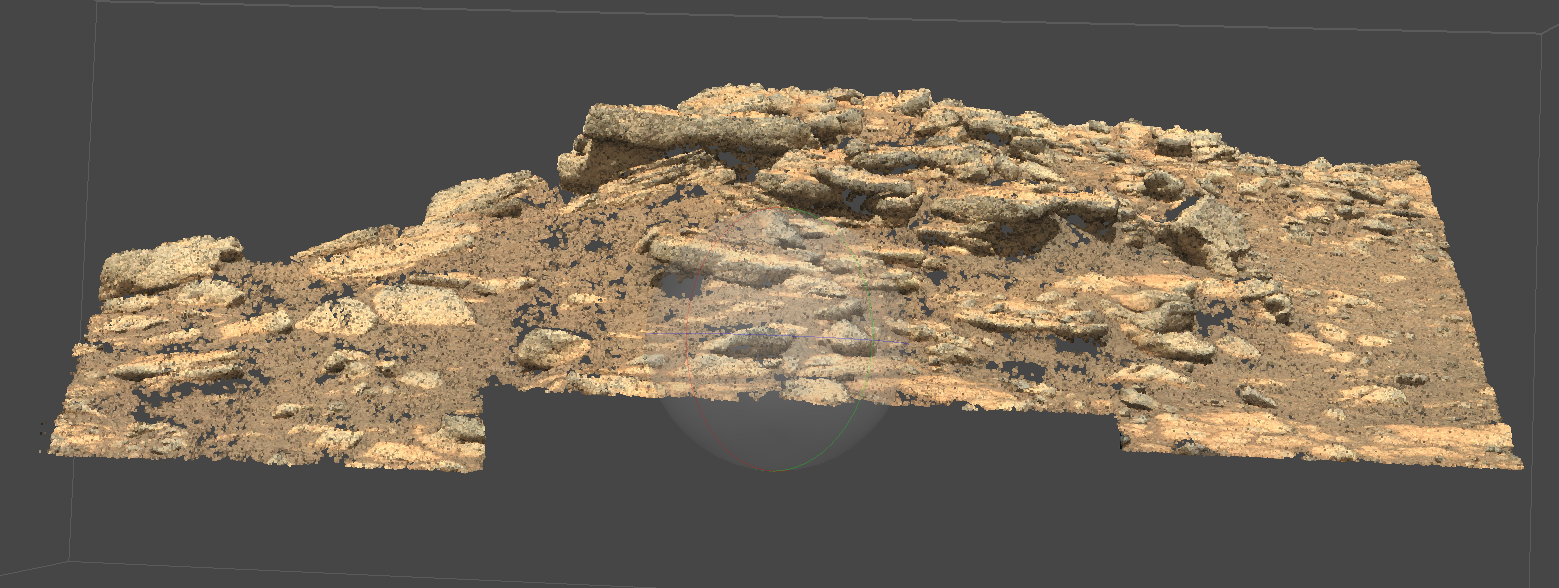
\includegraphics[scale=0.3]{img/sol2283.png}
	\label{fig:sol283}
	\caption{}
\end{figure}

\subsection{Callibrated}

\subsubsection{Sol-268}

Reconstruction of a drill made by rover with 4 Mastcam images. We included the parameters for the images which gave a good reconstruction and to produce an actual scale of the region unlike in \ref{sec:drilluncal}. Including the extrinsics gives the correct orientation of the area and the location of the object.

\begin{figure}[H]
	\centering
	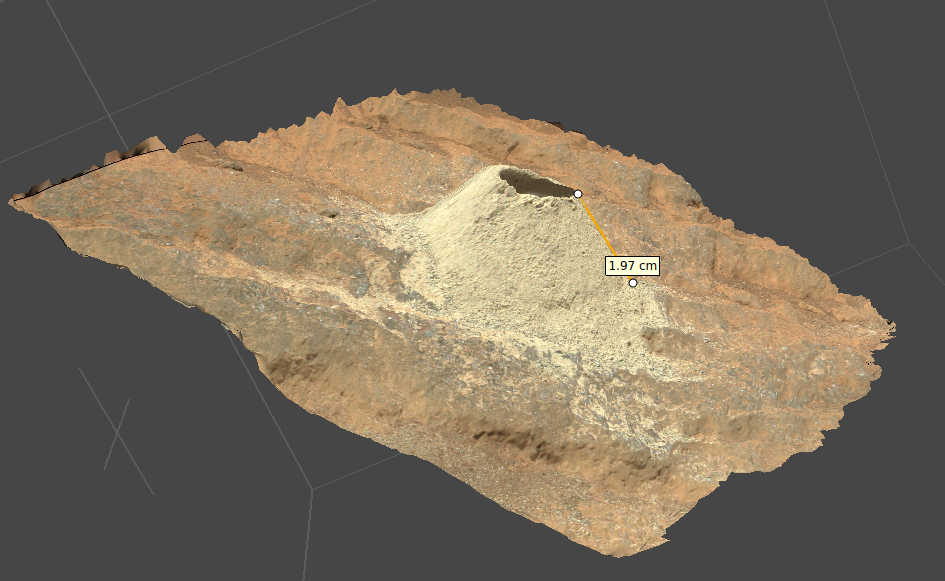
\includegraphics[scale=0.3]{img/drill.png}
	\label{fig:sol268calib}
	\caption{}
\end{figure}
\subsubsection{Sol-54}

In this Reconstruction of sol 54 we included the intrinsic and the extrinsics parameters in the agisoft with the same number of images as \ref{sec:sol54}. This gave us the correct orientation of the area.


\begin{figure}[H]
	\centering
	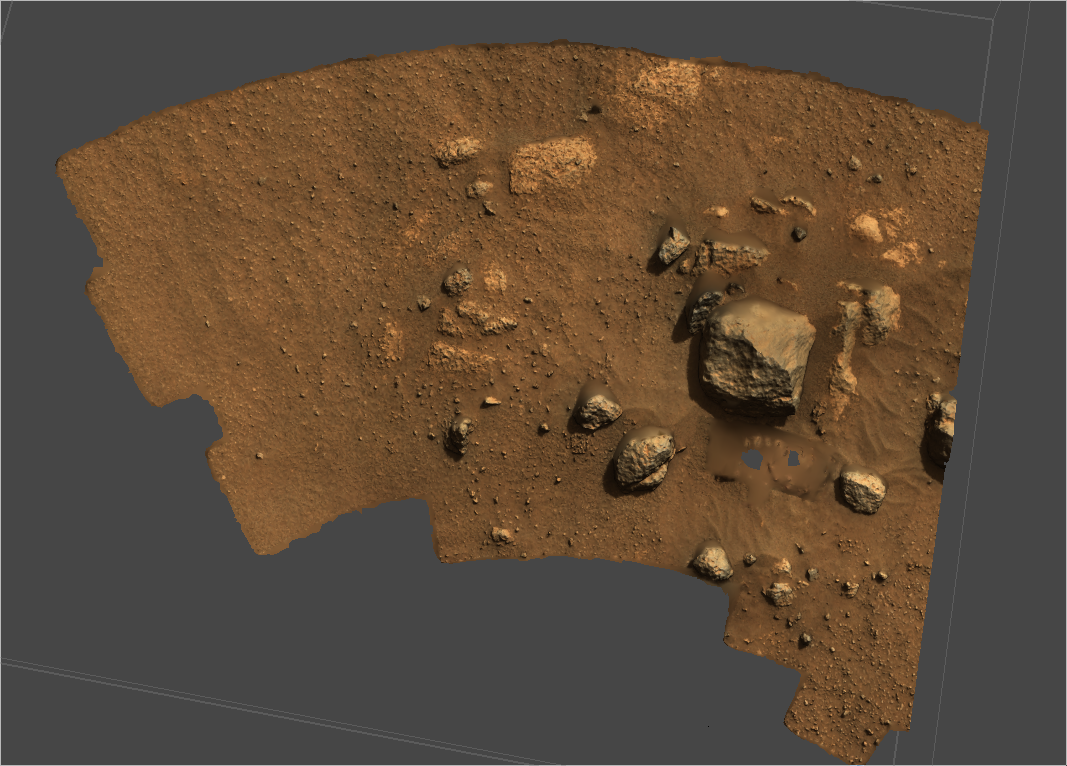
\includegraphics[scale=0.3]{img/sol54calib.png}
	\label{fig:sol54calib}
	\caption{}
\end{figure}

\subsubsection{Sol-283}

This sol was a considerably newer region which the rover was set to explore. Comparing with the Uncalibrated reconstruction the orientation in the Callibrated reconstruction was more accurate. We used 8 images from the Mastcam for the reconstruction. 


\begin{figure}[H]
	\centering
	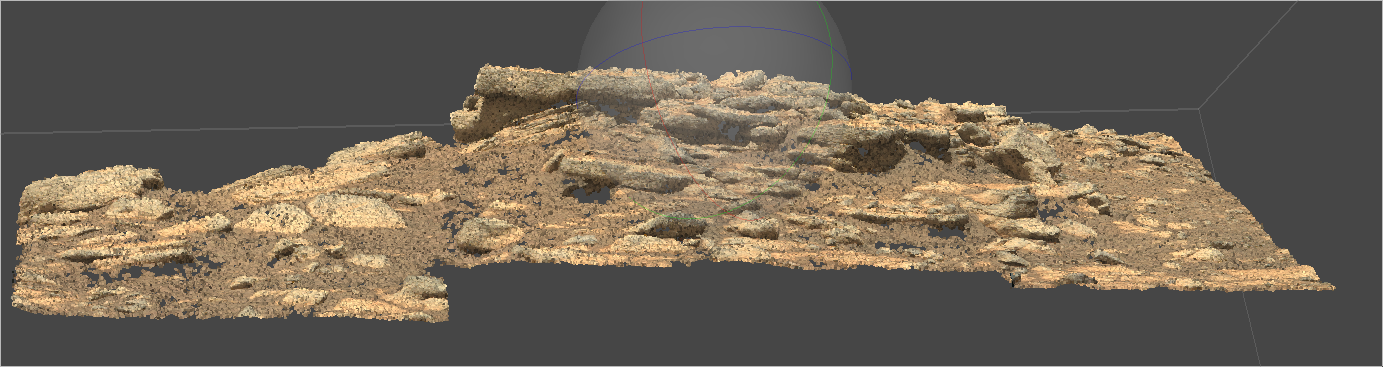
\includegraphics[scale=0.3]{img/sol283calib.png}
	\label{fig:sol283calib}
	\caption{}
\end{figure}




\newpage
\chapter{Conclusion and Outlook}

\appendix


%%%%%%%%%%%%%%%%%%%%%%%%%%%%%%%%%%%%%%%%%%%%%%%%%%%%%%%%%%%%%%%%%%%%%%%%%%%%%%%%%%%%%%%%%%%%%%%%%%%%%%%
%%%%%%%%%%%%%%%%%%%%%%%%%%%%%%%%%%%%%%%%%%%%%%%%%%%%%%%%%%%%%%%%%%%%%%%%%%%%%%%%%%%%%%%%%%%%%%%%%%%%%%%

\selectlanguage{english}

% Stil f�r Literaturverzeichnis
%\bibliographystyle{alpha}
%\bibliographystyle{apalike}
%\bibliographystyle{plainnat}
%\bibliographystyle{dinat}
\bibliographystyle{unsrtnat}
%\bibliographystyle{apasoft}

%Literaturverzeichniss
\bibliography{bib/literatur}


%%%%%%% MAYBE APPENDIX IF WE WANT TO ATTACH THE CODE OR SOMETHING LIKE THAT %%%
%\newpage
%\appendix
%\input{Anhang.tex}t



\setcounter{page}{1}
\pagenumbering{roman}
\listoffigures
\listoftables
\clearpage{\pagestyle{empty}\cleardoublepage}
% Seitenstil anpassen
\fancypagestyle{plain}{
% Alte Werte l�schen
\fancyhead{}
\fancyfoot{}
\renewcommand{\headrulewidth}{0pt}
}
\pagestyle{plain}


\end{document}
